\documentclass{article}
\usepackage[utf8]{inputenc}
\usepackage[bottom]{footmisc}
\usepackage{dirtytalk}
\usepackage{indentfirst}
\usepackage{mathtools}
\usepackage{amsmath}
\usepackage{amssymb}
\usepackage{graphicx}
\usepackage{mwe}
\usepackage{float}
\graphicspath{{Images/}}

\setlength{\oddsidemargin}{0in}
\setlength{\textwidth}{6.5in}
\setlength{\topmargin}{-.55in}
\setlength{\textheight}{9in}
\pagestyle{empty}


\title{ODE Models for a Parachutist's Fall}
\author{Adele Griffin, Zane Hall, Michael Nameika, Samantha Turner}
\date{}

\begin{document}

\maketitle

\section*{Introduction}


    The models represented below illustrate the path a skydiver will take as they travel to the Earth. This occurs in three stages that can be represented by a period of free-fall, the deployment of the parachute, and a descent with the parachute fully deployed. While mathematically representing all these pertinent pieces, we also must include specific factors that maintain safety for the parachutist. To model something that can be accurately applied in the real world you will see slight changes or assumptions made to account for the real-life events that happen during the experience of parachuting. We hope to portray this parachuting event using ordinary differentiation, accurate representations of gravity and air resistance, as well as explaining the process in such a way that is easily digestible by the common reader.

\section*{Problem Set-Up}


    Using Newton's Second Law of Motion, which states \say{The acceleration of an object depends on the mass of the object and the amount of force applied} (NASA), along with the assumption that air resistance is linearly proportional to velocity, we have depicted the phenomenon of the parachutist's flight with the following criteria:

    To begin, velocity of the parachutist is represented by the differential equation
    \begin{equation}
        \frac{dv}{dt} = -g - \frac{k}{m}v
    \end{equation}
    where $g$ is the acceleration due to gravity, $m$ is the mass of the falling body, and $k$ is the coefficient of air resistance. For our analysis, we assume $m = 5 \text{ slugs }$, with $1 \text{ slug} = 32.17 \text{ lbs}$, $g = 32/17 \text{ft/s}^2$. For constant air resistance, we have the following explicit forms of velocity and position with respect to time:
    \begin{align}
        v(t) &= -\frac{mg}{k} + \left(v_0 + \frac{mg}{k}\right)e^{-kt/m} \\
        h(t) &= -\frac{mg}{k}t - \frac{m}{k}\left(v_0 + \frac{mg}{k}\right)e^{-kt/m} + \frac{m}{k}\left(v_0 + \frac{mg}{k}\right) + h_0
    \end{align}
    where $v_0$ is the initial velocity and $h_0$ is the initial height of the parachutist. For our problem, we have $h_0 = 4000$ ft, and $v_0 = 0$, which means the parachutist "falls" out of the plane initially. We are also given that the terminal velocity $\left(-\frac{mg}{k}\right)$ is 176 ft/s. We are also given that the parachute will take 3 seconds to fully deploy, and we assume that the parachutist will deploy the parachute at approximately 3000 feet. We will investigate three different models for the coefficient of air resistance after the parachute is deployed: an instantaneous change, linear change, and a smooth change.

\section*{Stage 1: Free-Fall}

    The first portion of this problem consists of a free-fall for the skydiver, which describes the scenario in which gravity is the only force acting on the skydiver. After stepping out of the plane at 4000 ft, they will fall to the Earth with a maximum (terminal) velocity of 176 ft/s. The diver will need to pull the parachute at the safe height of 3000 ft above the ground (Wisconsin Skydiving Center). The parachutist will be in free-fall for 10.2 seconds before deploying the chute at 3000 feet above the ground. Therefore, $t_d = 10.2$ seconds. At this time, they will have a velocity of $-147.94$ ft/s. Using these parameters and the equations 2 and 3, we find the following plots for position and velocity of the skydiver before parachute deployment.

    Using $v(t)$ and a mass of 5 slugs for the skydiver, the air resistance when there is no parachute deployed and when one is deployed is $k_{np} = 0.92$ and $k_p = 10.44$, respectively.
    \begin{figure}[h]
        \centering
        \begin{minipage}{0.45\textwidth}
            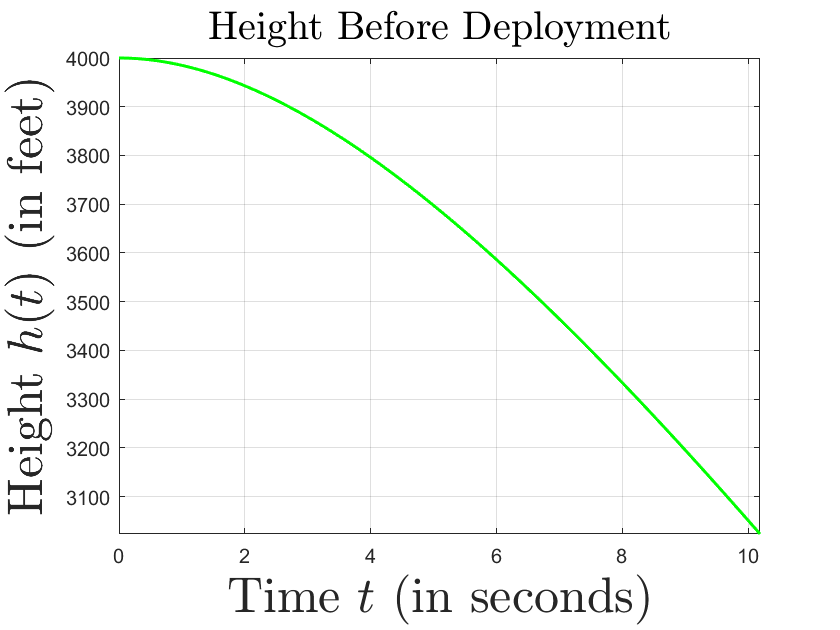
\includegraphics[scale = 0.35]{positionBeforeDeployment}
            \caption{Position of skydiver before parachute deployment}
        \end{minipage}\hfill
        \begin{minipage}{0.45\textwidth}
            \centering
            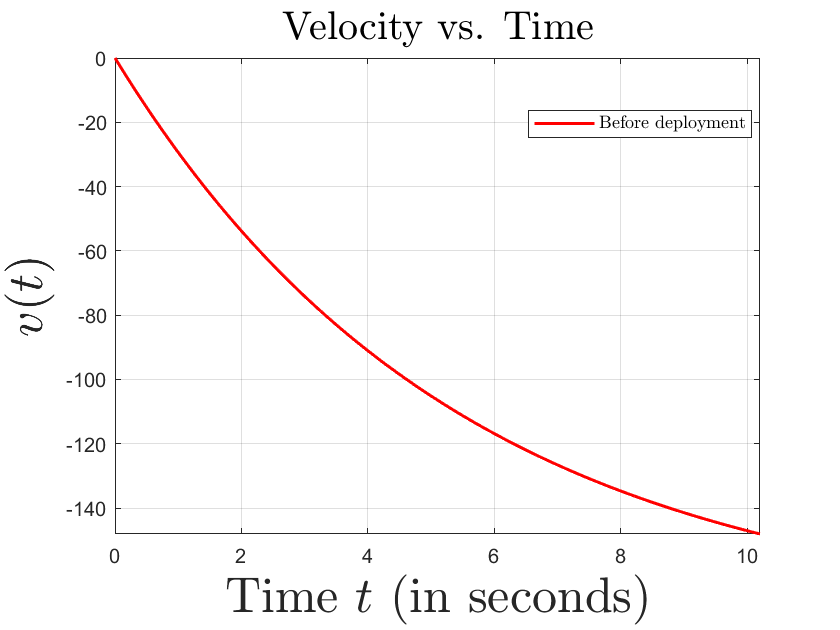
\includegraphics[scale = 0.35]{velocityBeforeDeployment}
            \caption{Velocity of skydiver before parachute deployment}
        \end{minipage}
    \end{figure}

    \section*{Stage 2: Deployment of the Parachute}
    Once the skydiver deploys the parachute, it takes approximately 3 seconds to fully deploy. During this time, the skydiver will experience the phenomenon known as jerk. The jerk is \say{the shock produced while the parachute deploys} (Meade). It can be expressed mathematically by the time derivative of acceleration:
    \begin{equation}
        j(t) = \frac{da}{dt} = -\frac{k'(t)}{m}v(t) - \frac{k(t)}{m}a(t)
    \end{equation}
    
    In this section, we compare three models for the coefficient of air resistance during the deployment of the parachute. To begin, we will assume the air resistance instantly changes from $k_{np}$ to $k_p$. That is, we may model the air resistance by
    \[k(t) = (k_p - k_{np})H(t - t_d) + k_{np}\]
    where $H(t)$ is the Heaviside step function. Notice that 
    \[k'(t) = (k_p - k_{np})\delta(t - t_d)\]
    where $\delta(t)$ is the Dirac delta function. Then the jerk at the time of deployment is infinite, which is not safe for the parachutist! The following figures show the air resistance, position, and velocity of the parachutist:
    \begin{figure}[H]
        \centering
        \begin{minipage}{0.45\textwidth}
            \centering
            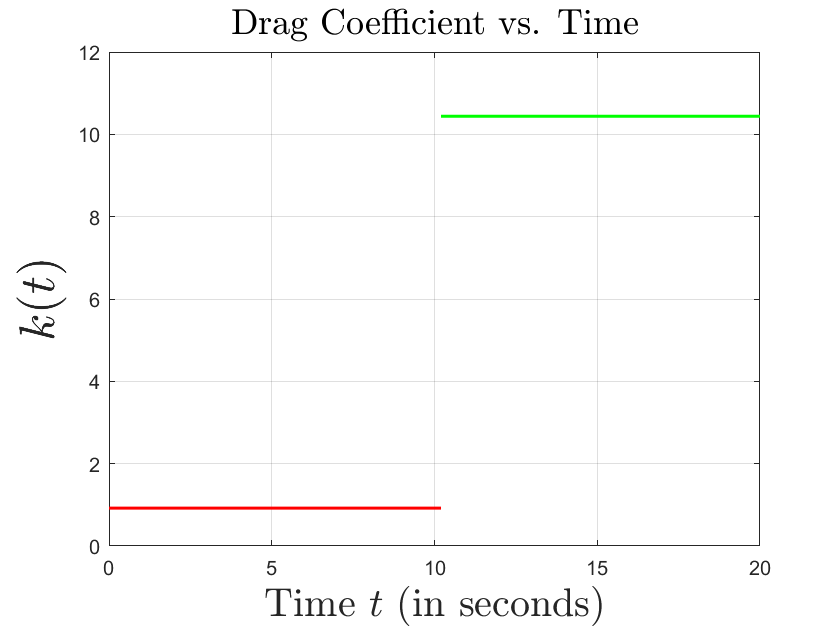
\includegraphics[scale = 0.45]{instantkplot}
            \caption{Coefficient of drag. Note the discontinuity at $t_d$.}
        \end{minipage}

        
        \begin{minipage}{0.45\textwidth}
            \centering
            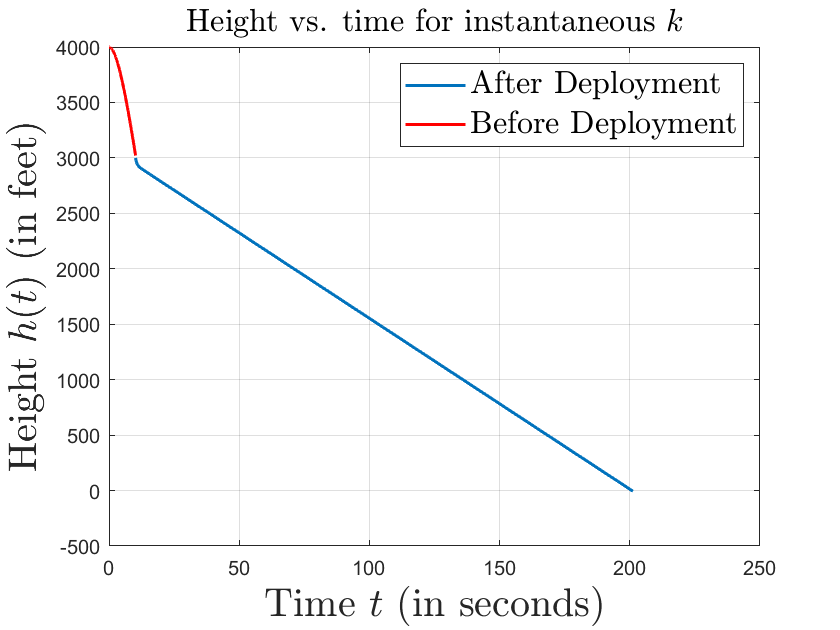
\includegraphics[scale = 0.35]{heightInstantK}
            \caption{Position of parachutist with instant change in $k$}
        \end{minipage}
        \begin{minipage}{0.45\textwidth}
            \centering
            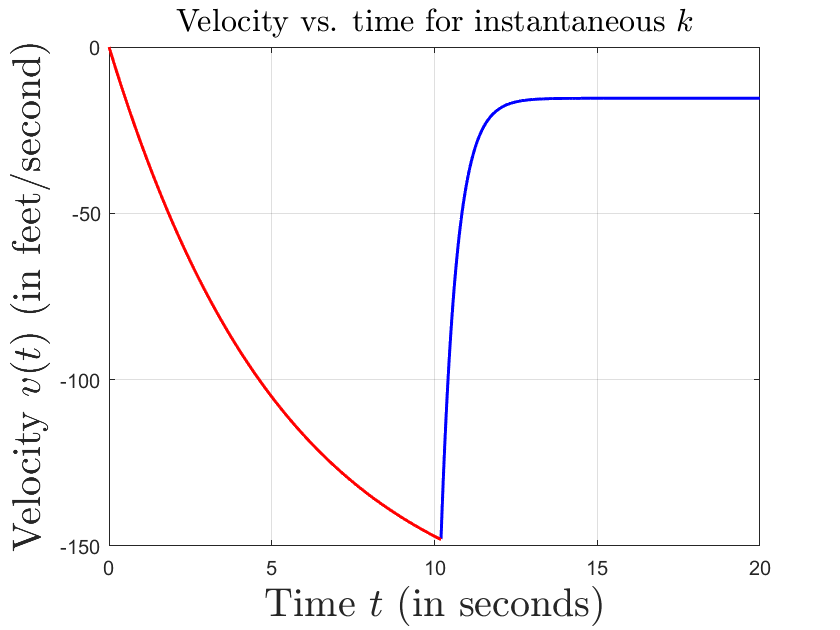
\includegraphics[scale = 0.35]{velocityInstantK}
            \caption{Velocity of parachutist with instant change in $k$.}
        \end{minipage}
    \end{figure}
    With this model, our parachutist experiences infinite jerk at the time of parachute deployment!
    \newline

    Now, let us inspect the case of a linear fit between $k_{np}$ and $k_p$. During the parachute deployment, we find the following linear function for the drag coefficient:
    \[k_d(t) = \frac{k_p - k_{np}}{3}(t - t_d) + k_{np}\]
    Using this, we have the following plots for the drag coefficient, height, and velocity:
    \begin{figure}[H]
        \centering
        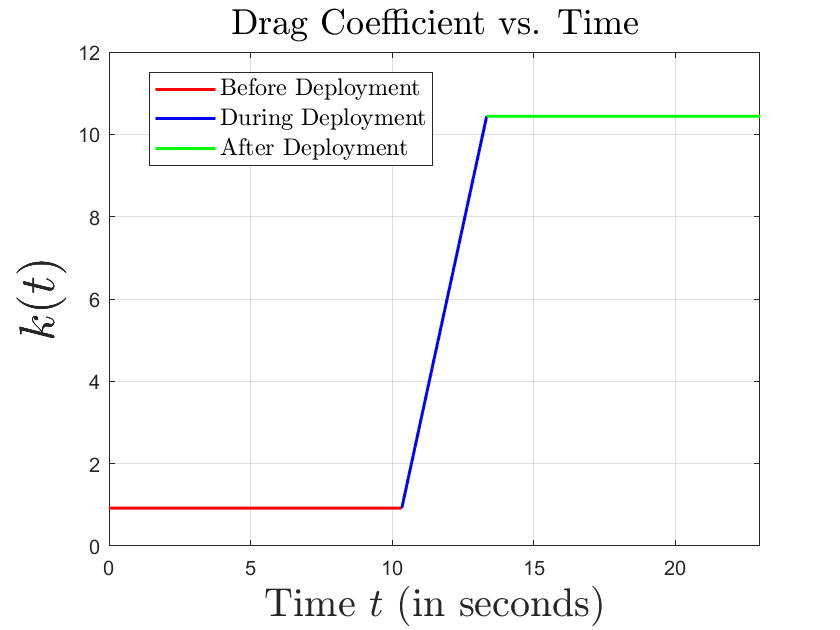
\includegraphics[scale = 0.45]{linearkplot}
        \caption{Linear drag coefficient fit}
    \end{figure}
    
    \begin{figure}[H]
        \centering
        \begin{minipage}{0.45\textwidth}
            \centering
            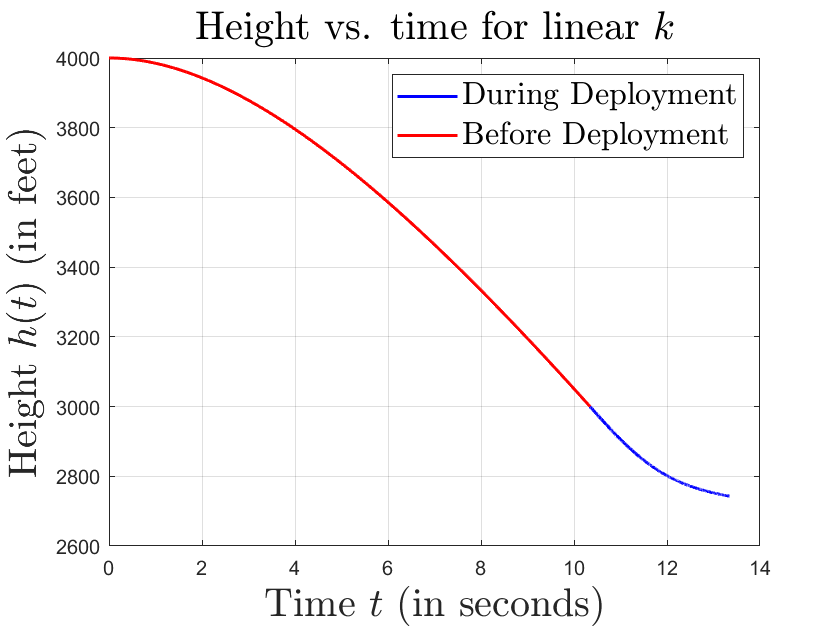
\includegraphics[scale = 0.35]{heighlineark}
            \caption{Height of parachutist with linear $k$}
        \end{minipage}
        \begin{minipage}{0.45\textwidth}
            \centering
            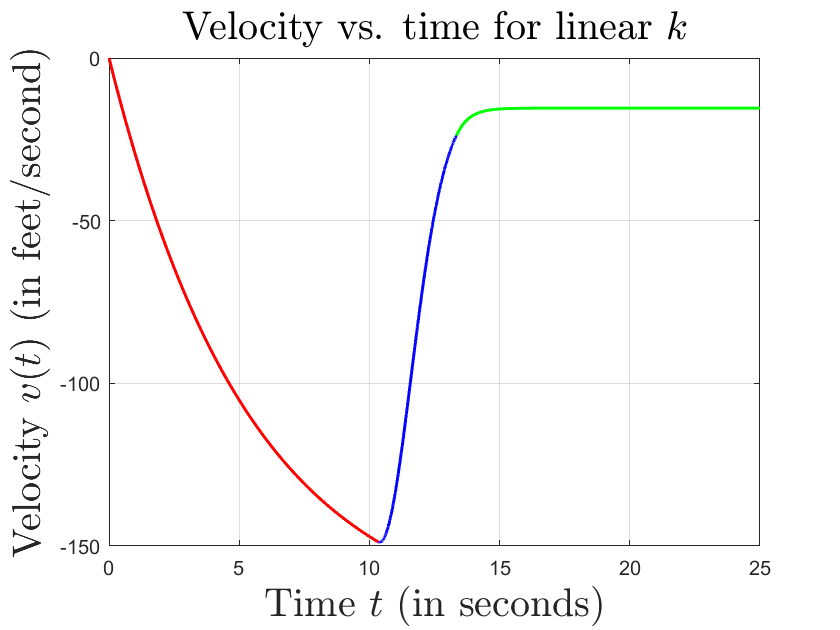
\includegraphics[scale = 0.35]{velocitylineark}
            \caption{Velocity of parachutist with linear $k$}
        \end{minipage}
    \end{figure}
    Similar to the instantaneous change in $k$ model, the linear model presents a problem in that the derivative of $k$ does not exist at $t_d$ and $t_d + 3$. This means the jerk is undefined at the beginning and end of the parachute deployment.
    \newline

    Now let us inspect a model where we connect $k_{np}$ and $k_p$ with a cubic spline (a smooth curve fit). This fit is represented by the smooth blue line in figure 9. The endpoints and the derivatives at the endpoints match the air resistance before and after the parachute is deployed.
    \begin{figure}[H]
        \centering
        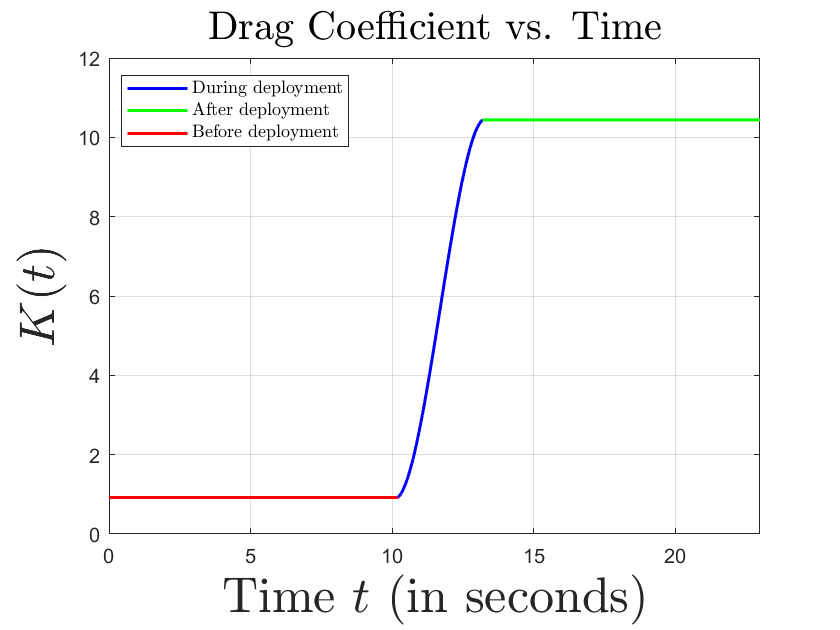
\includegraphics[scale = 0.45]{drag coefficient plot}
        \caption{Drag coefficient with smooth fitting curve}
    \end{figure}

    Now that $k$ is smooth, we can look at the jerk during deployment, along with the velocity of the parachutist, as depicted in the following figures:
    \begin{figure}[H]
        \centering
        \begin{minipage}{0.45\textwidth}
            \centering
            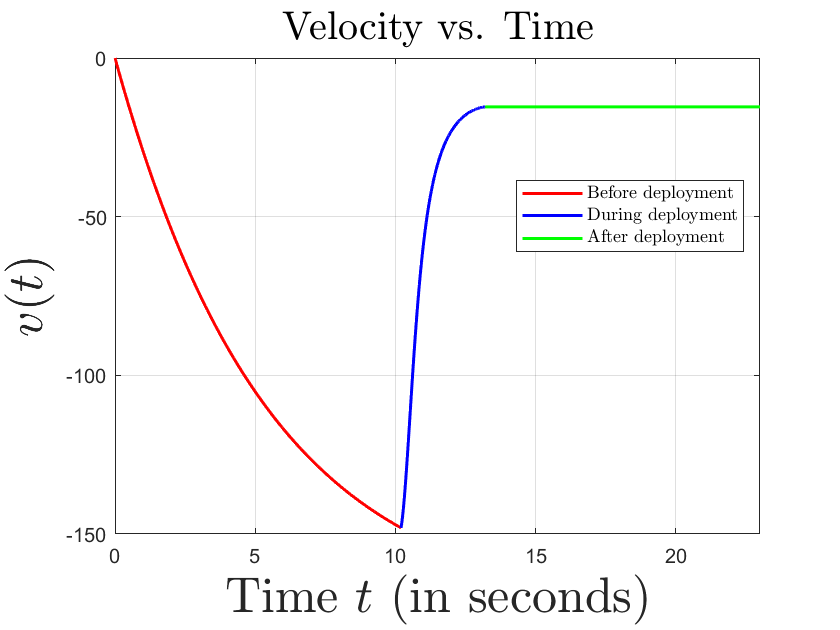
\includegraphics[scale = 0.4]{velocity plot cubic}
            \caption{Velocity of parachutist with smooth $k$}
        \end{minipage}
        \begin{minipage}{0.45\textwidth}
            \centering
            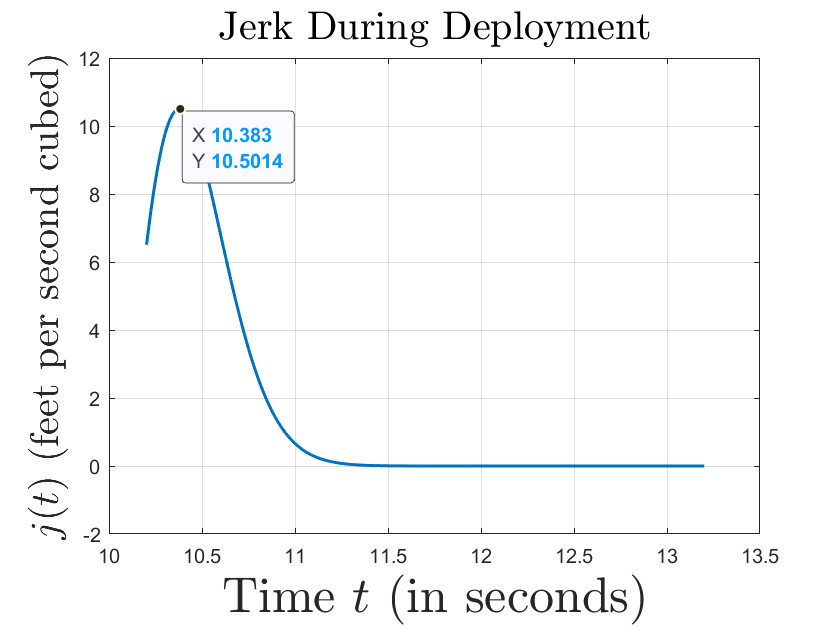
\includegraphics[scale = 0.4]{jerk plot}
            \caption{Jerk with smooth $k$}
        \end{minipage}
        
    \end{figure}

    The highlighted point shows the maximum jerk during parachute deployment, which corresponds to a jerk of approximately $1.64 \text{ g/s}$, well below our maximum $3 \text{ g/s}$. Our parachutist is safe!

    \section*{Stage 3: Open Parachute}

    The last portion of this problem deals with the parachutist after their parachute has been fully deployed. We know that they cannot land at a rate faster than the equivalent velocity of stepping off a 5' tall object. We arrived at this speed by using the same values for terminal velocity, 176 ft/s, as well as the same physical equations that consider air-resistance. From here we arrived at the fact that the maximum velocity was -17.355 ft/s. We accounted for additional safety measures, as well as utilizing the $k_p$ value and decided to limit the maximum velocity to -15.41 ft/s. With the maximum velocity set at -15.41 ft/s, and the work from Stage 2, we can also note that $v_0 = -15.41$ ft/s for this portion of the problem.
    \newline
    
    For this stage, equation (1) is used with $v_0 = -15.41$ ft/s, $h_0 = 2861.31$, and terminal velocity equal to $-15.41$ ft/s. This gives a simpler equation that explains that the time it will take to reach the ground once the chute is open is proportional to $\frac{h_0}{15.41 \text{ ft/s}}$. This gives us a landing time of 185.88 seconds. Therefore, once the chute is fully deployed, the skydiver will fall for an additional 185.88 seconds.

    \begin{figure}[H]
        \centering
        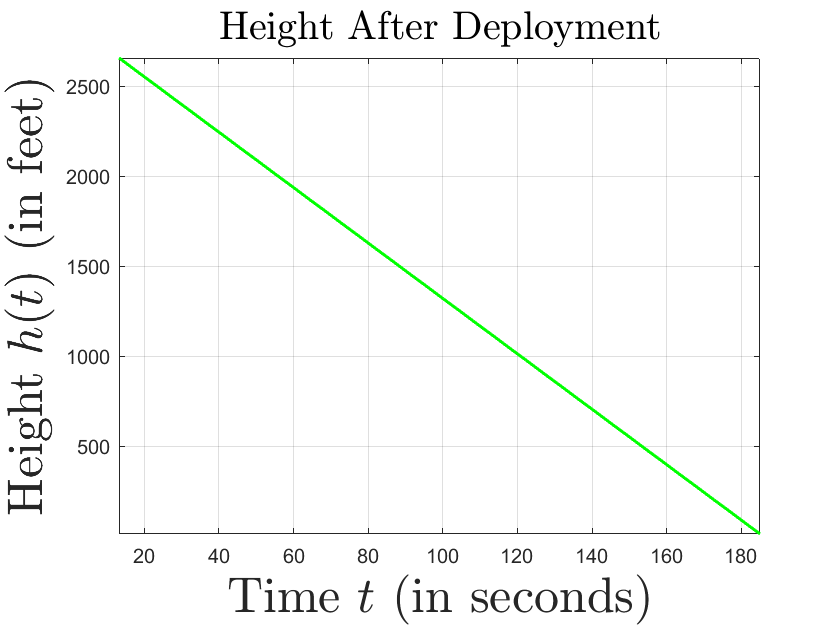
\includegraphics[scale = 0.45]{heightAfterDeployment}
        \caption{The height of the parachutist after the parachute is fully deployed}
    \end{figure}


    \section*{Conclusion}
    As demonstrated, a skydiver who exits a plane 4000 feet above the Earth takes approximately 198.88 seconds to reach the ground, or approximately 3.31 minutes. They will be in free-fall for 10.2 seconds and deploy the parachute at 3000 feet while travelling at a velocity of -147.94 ft/s. The jerk when deploying the parachute does not exceed $10.50 \text{ ft/s}^3$, which is equivalent to approximately 1.64 g's of force per second. The parachute takes three seconds to fully deploy, and the end velocity of the skydiver is -15.41 ft/s. Finally, the parachute is fully deployed at 2861.31 feet and the skydiver will fall at a velocity of -15.41 ft/s for a total of 185.88 seconds to reach the ground.

    \newpage
    \section*{Cited Sources}
    Meade, Douglas B. “ODE Models for the Parachute Problem.” SIAM Review, vol. 40, no. 2, 1998, pp. 327–332.  
    \newline

NASA. (2022, October 27). Newton's laws of motion - Glenn Research Center. NASA. Retrieved February 2, 2023, from https://www1.grc.nasa.gov/beginners-guide-to-aeronautics/newtons-laws-of-motion/  
\newline

Wisconsinskydivingcenter. “What Is the Average Skydiving Height?” Wisconsin Skydiving Center, 12 July 2021, https://wisconsinskydivingcenter.com/blog/what-is-the-average-skydiving-height/. 
\end{document}
